\section{Attention-based Decoding Sequences}
\begin{frame}{Decoding Sequences with Attention}
  \textbf{Attention-Based Decoding -- Overview}
  \begin{itemize}
    \item[$\blacktriangleright$]
      The decoder uses attention to select relevant encoder hidden states at each decoding step.
  \end{itemize}
  \textbf{Combines:}
  \begin{itemize}
    \item[] $\bullet$ Previous decoder state
    \item[] $\bullet$ Encoder hidden states
    \item[] $\bullet$ Attention context vector
  \end{itemize}
  \begin{itemize}
    \item[$\blacktriangleright$]
      The output at time $t$:
      \begin{equation*}
        y_t = \mathrm{Decoder}(y_{t-1}, \text{context}_t)
      \end{equation*}
  \end{itemize}
\end{frame}

% Slide 33
  \begin{frame}{Attention-Based Decoding}
  \centering
  
\includegraphics[width=0.5\paperwidth,height=0.5\paperheight,keepaspectratio]{assets/Lecture-5_Attention_Mechanism_Deep_Dive/pdf_page_033.png}\end{frame}

% Slide 34
\begin{frame}{Decoding - Steps}
  \begin{enumerate}
    \item \textbf{Compute query}: Generate a query vector from the current decoder hidden state.
    \item \textbf{Align with encoder outputs}: Compare the query with encoder outputs (keys) to measure relevance.
    \item \textbf{Get attention weights}: Apply softmax to the alignment scores to obtain attention weights.
    \item \textbf{Compute context}: Calculate the context vector as the weighted sum of encoder outputs using the attention weights.
    \item \textbf{Feed into decoder}: Use the context vector and previous outputs as input for the next decoding step.
  \end{enumerate}
\end{frame}

% Slide 35
\begin{frame}{Attention}
  \centering
  
\includegraphics[width=0.5\paperwidth,height=0.5\paperheight,keepaspectratio]{assets/Lecture-5_Attention_Mechanism_Deep_Dive/pdf_page_035.png}\end{frame}

% Slide 36
\begin{frame}{Attention}
  \centering
  
\includegraphics[width=0.5\paperwidth,height=0.5\paperheight,keepaspectratio]{assets/Lecture-5_Attention_Mechanism_Deep_Dive/pdf_page_036.png}\end{frame}

% Slide 37
\begin{frame}{Attention}
  \centering
  
\includegraphics[width=0.5\paperwidth,height=0.5\paperheight,keepaspectratio]{assets/Lecture-5_Attention_Mechanism_Deep_Dive/pdf_page_037.png}\end{frame}

% Slide 38
\begin{frame}{Attention}
  \centering
  
\includegraphics[width=0.5\paperwidth,height=0.5\paperheight,keepaspectratio]{assets/Lecture-5_Attention_Mechanism_Deep_Dive/pdf_page_038.png}\end{frame}

% Slides 46--56 from lec19.transformers.pdf as pdf_page_039.png--049.png
\begin{frame}{Attention}
  \centering
  
\includegraphics[width=0.5\paperwidth,height=0.5\paperheight,keepaspectratio]{assets/Lecture-5_Attention_Mechanism_Deep_Dive/pdf_page_039.png}
\end{frame}

% Slide 40
\begin{frame}{Attention}
  \centering
  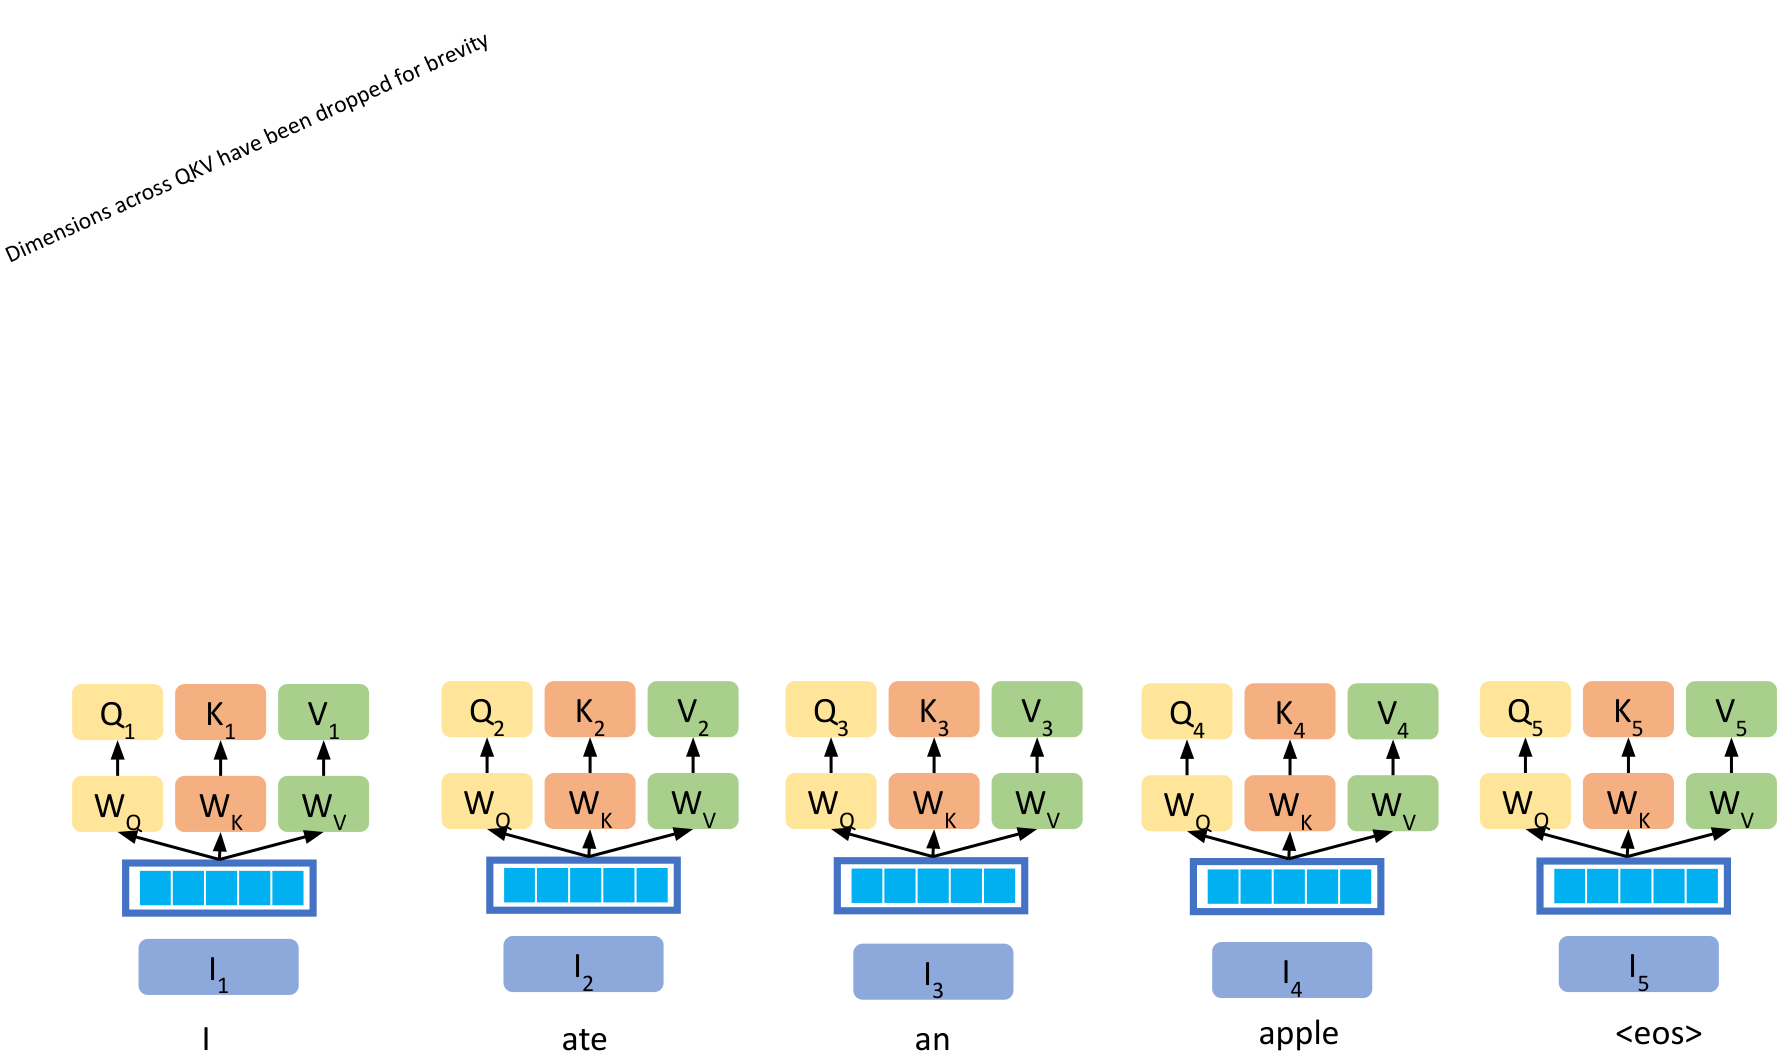
\includegraphics[width=0.5\paperwidth,height=0.5\paperheight,keepaspectratio]{assets/Lecture-5_Attention_Mechanism_Deep_Dive/pdf_page_040.png}
\end{frame}

% Slide 41
\begin{frame}{Attention}
  \centering
  
\includegraphics[width=0.5\paperwidth,height=0.5\paperheight,keepaspectratio]{assets/Lecture-5_Attention_Mechanism_Deep_Dive/pdf_page_041.png}
\end{frame}

% Slide 42
\begin{frame}{Attention}
  \centering
  
\includegraphics[width=0.5\paperwidth,height=0.5\paperheight,keepaspectratio]{assets/Lecture-5_Attention_Mechanism_Deep_Dive/pdf_page_042.png}
\end{frame}

% Slide 43
\begin{frame}{Attention}
  \centering
  
\includegraphics[width=0.5\paperwidth,height=0.5\paperheight,keepaspectratio]{assets/Lecture-5_Attention_Mechanism_Deep_Dive/pdf_page_043.png}
\end{frame}

% Slide 44
\begin{frame}{Attention}
  \centering
  
\includegraphics[width=0.5\paperwidth,height=0.5\paperheight,keepaspectratio]{assets/Lecture-5_Attention_Mechanism_Deep_Dive/pdf_page_044.png}
\end{frame}

% Slide 45
\begin{frame}{Attention}
  \centering
  
\includegraphics[width=0.5\paperwidth,height=0.5\paperheight,keepaspectratio]{assets/Lecture-5_Attention_Mechanism_Deep_Dive/pdf_page_045.png}
\end{frame}

% Slide 46
\begin{frame}{Attention}
  \centering
  
\includegraphics[width=0.5\paperwidth,height=0.5\paperheight,keepaspectratio]{assets/Lecture-5_Attention_Mechanism_Deep_Dive/pdf_page_046.png}
\end{frame}

\begin{frame}{Attention}
  \centering
  
\includegraphics[width=0.5\paperwidth,height=0.5\paperheight,keepaspectratio]{assets/Lecture-5_Attention_Mechanism_Deep_Dive/pdf_page_047.png}
\end{frame}

% Slide 48
\begin{frame}{Attention}
  \centering
  
\includegraphics[width=0.5\paperwidth,height=0.5\paperheight,keepaspectratio]{assets/Lecture-5_Attention_Mechanism_Deep_Dive/pdf_page_048.png}
\end{frame}

% Slide 49
\begin{frame}{Attention}
  \centering
  
\includegraphics[width=0.5\paperwidth,height=0.5\paperheight,keepaspectratio]{assets/Lecture-5_Attention_Mechanism_Deep_Dive/pdf_page_049.png}
\end{frame}

% Slide 50
\begin{frame}{Attention}
  \centering
  
\includegraphics[width=0.5\paperwidth,height=0.5\paperheight,keepaspectratio]{assets/Lecture-5_Attention_Mechanism_Deep_Dive/pdf_page_050.png}
\end{frame}

% Slide 51
\begin{frame}{Attention}
  \centering
  
\includegraphics[width=0.5\paperwidth,height=0.5\paperheight,keepaspectratio]{assets/Lecture-5_Attention_Mechanism_Deep_Dive/pdf_page_051.png}
\end{frame}

% Slide 52
\begin{frame}{Attention}
  \centering
  
\includegraphics[width=0.5\paperwidth,height=0.5\paperheight,keepaspectratio]{assets/Lecture-5_Attention_Mechanism_Deep_Dive/pdf_page_052.png}\end{frame}

% \begin{frame}[plain]
%   \centering
%   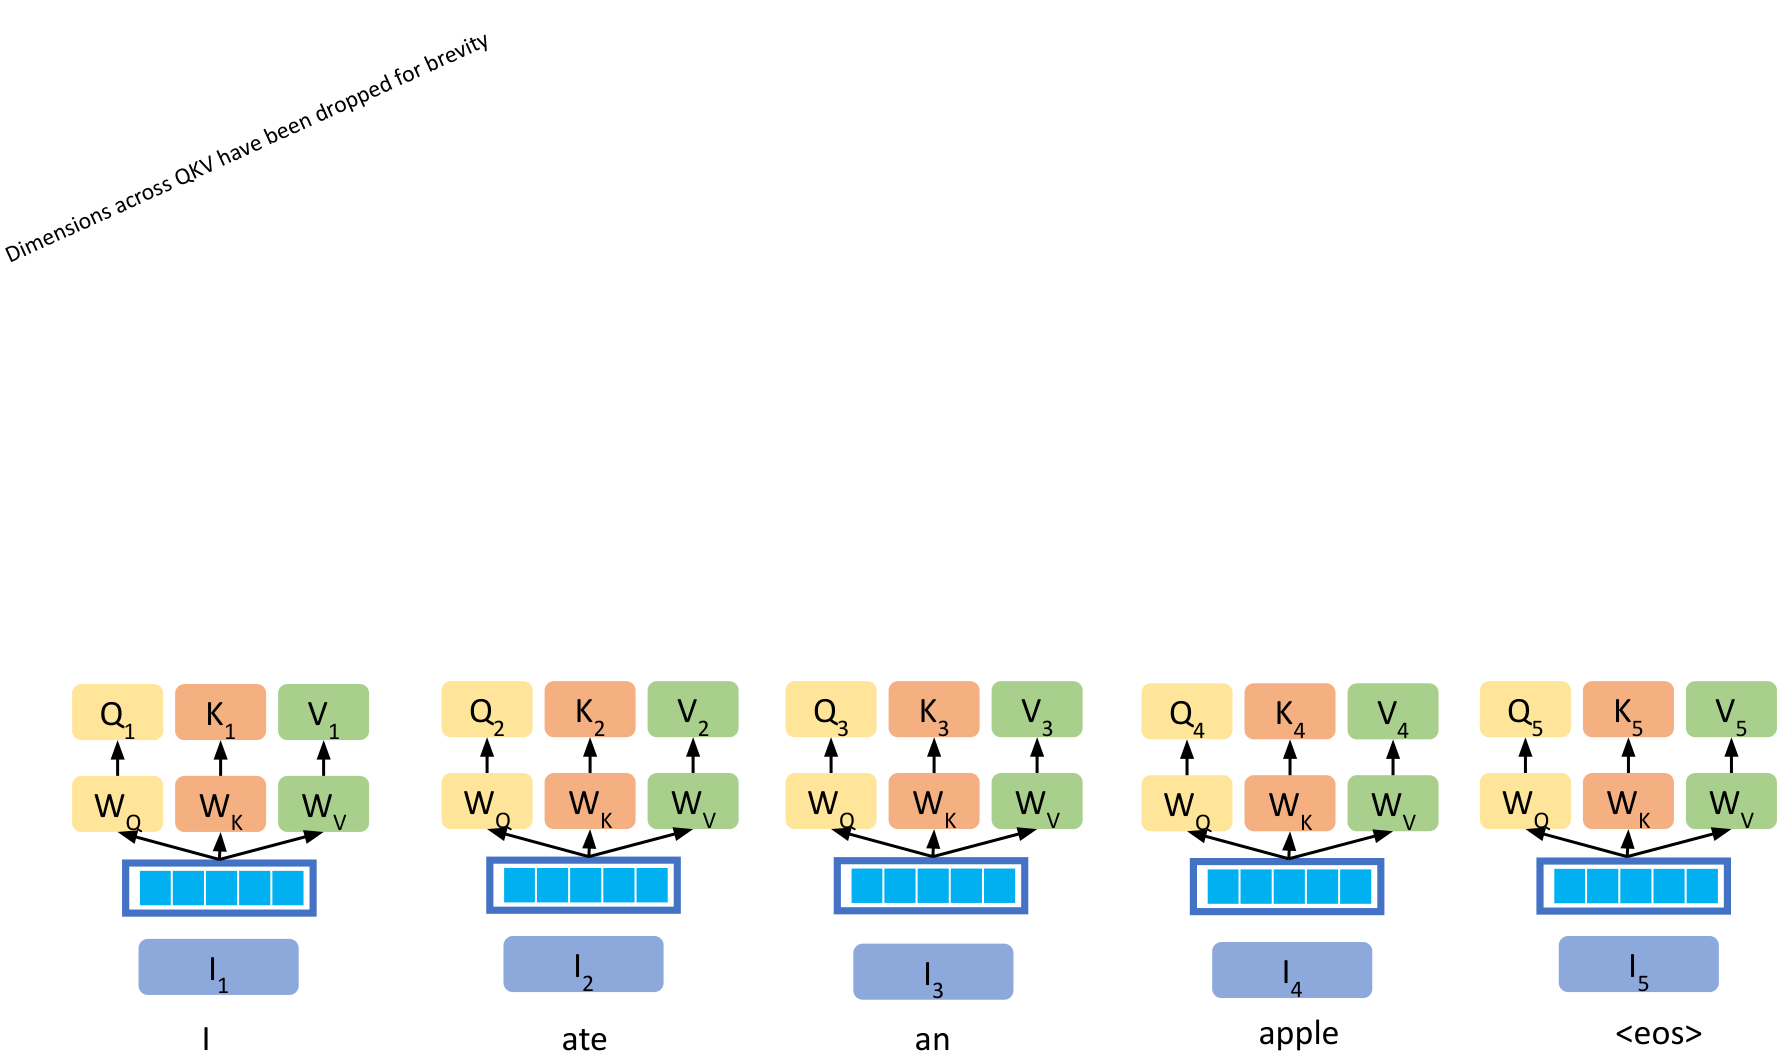
\includegraphics[width=0.5\paperwidth,height=0.5\paperheight,keepaspectratio]{assets/Lecture-5_Attention_Mechanism_Deep_Dive/pdf_page_040.png}\end{frame}

% \begin{frame}[plain]
%   \centering
%   
\includegraphics[width=0.5\paperwidth,height=0.5\paperheight,keepaspectratio]{assets/Lecture-5_Attention_Mechanism_Deep_Dive/pdf_page_041.png}\end{frame}

% \begin{frame}[plain]
%   \centering
%   
\includegraphics[width=0.5\paperwidth,height=0.5\paperheight,keepaspectratio]{assets/Lecture-5_Attention_Mechanism_Deep_Dive/pdf_page_042.png}\end{frame}

% \begin{frame}[plain]
%   \centering
%   
\includegraphics[width=0.5\paperwidth,height=0.5\paperheight,keepaspectratio]{assets/Lecture-5_Attention_Mechanism_Deep_Dive/pdf_page_043.png}\end{frame}

% \begin{frame}[plain]
%   \centering
%   
\includegraphics[width=0.5\paperwidth,height=0.5\paperheight,keepaspectratio]{assets/Lecture-5_Attention_Mechanism_Deep_Dive/pdf_page_044.png}\end{frame}

% \begin{frame}[plain]
%   \centering
%   
\includegraphics[width=0.5\paperwidth,height=0.5\paperheight,keepaspectratio]{assets/Lecture-5_Attention_Mechanism_Deep_Dive/pdf_page_045.png}\end{frame}

% \begin{frame}[plain]
%   \centering
%   
\includegraphics[width=0.5\paperwidth,height=0.5\paperheight,keepaspectratio]{assets/Lecture-5_Attention_Mechanism_Deep_Dive/pdf_page_046.png}\end{frame}

% \begin{frame}[plain]
%   \centering
%   
\includegraphics[width=0.5\paperwidth,height=0.5\paperheight,keepaspectratio]{assets/Lecture-5_Attention_Mechanism_Deep_Dive/pdf_page_047.png}\end{frame}

% \begin{frame}[plain]
%   \centering
%   
\includegraphics[width=0.5\paperwidth,height=0.5\paperheight,keepaspectratio]{assets/Lecture-5_Attention_Mechanism_Deep_Dive/pdf_page_048.png}\end{frame}

% \begin{frame}[plain]
%   \centering
%   
\includegraphics[width=0.5\paperwidth,height=0.5\paperheight,keepaspectratio]{assets/Lecture-5_Attention_Mechanism_Deep_Dive/pdf_page_049.png}\end{frame}

% \begin{frame}[plain]
%   \centering
%   
\includegraphics[width=0.5\paperwidth,height=0.5\paperheight,keepaspectratio]{assets/Lecture-5_Attention_Mechanism_Deep_Dive/pdf_page_050.png}\end{frame}

% \begin{frame}[plain]
%   \centering
%   
\includegraphics[width=0.5\paperwidth,height=0.5\paperheight,keepaspectratio]{assets/Lecture-5_Attention_Mechanism_Deep_Dive/pdf_page_051.png}\end{frame}

% \begin{frame}[plain]
%   \centering
%   
\includegraphics[width=0.5\paperwidth,height=0.5\paperheight,keepaspectratio]{assets/Lecture-5_Attention_Mechanism_Deep_Dive/pdf_page_052.png}\end{frame}

% Slide 53
\begin{frame}{Attention}
  \centering
  
\includegraphics[width=0.5\paperwidth,height=0.5\paperheight,keepaspectratio]{assets/Lecture-5_Attention_Mechanism_Deep_Dive/pdf_page_053.png}\end{frame}


% Slide 54
\begin{frame}{Decoding -- Example: Translation}
\textbf{Example: English to French Translation}

\vspace{0.7em}

\begin{itemize}
  \item[] \textbf{Source Sentence (English)}\\
  \textit{The cat sat on the mat.}
  \vspace{0.3em}
  \item[] \textbf{Target Sentence (French)}\\
  \textit{Le chat s'est assis sur le tapis.}
\end{itemize}

\vspace{0.4em}

\begin{itemize}
  \item[$\blacktriangleright$] At each decoding step, the decoder generates a French word by:
    \begin{enumerate}
      \item Using the current decoder hidden state.
      \item Attending to relevant English words via attention weights.
      \item Computing a context vector as a weighted sum of encoder outputs.
    \end{enumerate}
  \item[$\blacktriangleright$] For example, when generating ``\textit{chat}'', the attention focuses on ``cat''.
  \item[$\blacktriangleright$] The process repeats for each word, dynamically shifting attention.
\end{itemize}

\end{frame}
